\documentclass{article}
\usepackage{amsmath}
\usepackage[a4paper]{geometry}
\usepackage{graphicx}
\usepackage{caption}
\usepackage{subcaption}

\begin{document}

\author{
Oh Shunhao\\
  \texttt{A0065475X}
  \and
Nguyen Quoc Dat\\
  \texttt{A0116703N}
}
\title{CS4234: 2D Strip Packing - Interim Report}
\date{}

\maketitle

\begin{abstract}
\begin{center}
The 2D Strip Packing problem is concerned with the minimum height of a fixed-width strip needed to pack a set of rectangles into the strip. In this report, we give a brief summary of the current state-of-the art, and experiment with the practical effectiveness of some of the existing algorithms.
\end{center}
\end{abstract}

\section{Problem Definition}
In the Strip Packing problem, we are given an infinitely tall strip, of maximum width $W$, and a set of $n$ rectangles $s_1,s_2,\cdots,s_n$, each represented by a tuple $s_i = (w_i,h_i)$, representing the width and height of each rectangle.\\
\\
The task is to pack all of the $n$ rectangles into the strip, so that none of the rectangles overlap, and such that the total height of the strip is minimised.\\
\\
This problem has many applications in the industry, like in manufacturing, where rectangular pieces need to be cut out of a strip of fixed width, or perhaps in sprite packing for games, where fixed-size sprites can be packed into a single image to minimise the memory footprint of a game.\\

\section{State of the Art}
The decision problem of Strip Packing easily shown to be NP-HARD via a reduction from the partition problem.\\
\\
Assuming $P \neq NP$, there is no absolute polynomial time approximation scheme for Strip Packing. In fact, there is no algorithm with an absolute approximation ratio better than $\frac{3}{2} - \epsilon$ as 1-dimensional bin-packing is a subproblem of strip packing (1-dimensional bin packing is equivalent to strip packing with rectangles of height $1$), and in 1-dimensional bin packing, it is NP-HARD to distinguish whether OPT is $2$ or $3$ due to a reduction from the Partition problem.\\
\\
The current best known absolute approximation algorithm has an approximation ratio of $\frac{5}{3} + \epsilon$ by Harren et. al. \cite{harren1}, which is close to the lower bound of $\frac{3}{2} - \epsilon$. On the other hand, asymptotic approximation algorithms do much better. Simple algorithms like First-Fit Decreasing Height and Split-Fit already achieve asymptotic approximation ratios of $\frac{17}{10}$ and $\frac{3}{2}$ respectively. The best known asymptotic approximation ratio for Strip Packing is $\frac{5}{4}$ by Baker et. al.  \cite{baker1}.\\

\section{Existing algorithms}
Many existing approximation algorithms for 2-D Strip Packing are level-oriented algorithms. Level-oriented algorithms involve packing items into shelves of certain heights. These algorithms include First-Fit Decreasing Height, and Split-Fit.
\subsection{First-Fit Decreasing Height}
\textit{First-Fit Decreasing Height} (FFDH) places the rectangles in decreasing height order one by one on the bottom of the strip. When a rectangle cannot be placed on the bottom the strip, a new shelf is created from the top y-coordinate of the leftmost (tallest) rectangle of the topmost shelf.\\
\\
For a given list $L$ of rectangles, the performance of FFDH is bounded by the following:
\[
	FFDH(L) \leq 1.7 \times OPT(L) + 1
\]
The proof for the approximation ratio of FFDH is based on the proof of the approximation ratio for the First-Fit algorithm for the one-dimensional bin packing problem, which is also asymptotically 1.7-approximate.
\subsection{Split-Fit}
\textit{Split-Fit} (SF) also sorts the rectangles by decreasing height. We find $m \geq 1$, which is the maximum integer such that all given rectangles have width less than or equal to $\frac{1}{m}$. The rectangles are then divided into two sets $L_1$ and $L_2$:
\begin{itemize}
\item $L_1$ contains rectangles with width greater than $\frac{1}{m+1}$.
\item $L_2$ contains rectangles with width less than or equal to $\frac{1}{m+1}$.
\end{itemize}
Then, the rectangles in $L_1$ are packed using FFDH. The resulting shelves produced are then rearranged by width, such that all shelves with width more than $\frac{m+1}{m+2}$ are below shelves with width less than or equal to $\frac{m+1}{m+2}$. This results in a free rectangle $R$ of width $\frac{1}{m+2}$ to the right of the shelves with width less than or equal to $\frac{m+1}{m+2}$.\\
\\
We then proceed to pack rectangles in $L_2$ into R, treating it as a strip of width $\frac{1}{m+2}$. However, if a new shelf is to be created, and it exceeds the height of R, then it is placed on top of the shelves from $L_1$ with width less than or equal to $\frac{m+1}{m+2}$, and thus allows the full width of the original strip. This continues until all rectangles have been packed.\\
\\
The performance of SF is bounded by the value of $m$:
\[
	SF(L) \leq \frac{m+2}{m+1}OPT(L) + 2
\]
In other words, if all rectangles have width less than or equal to one third of the strip width, then $m = 3$, and thus the performance bound for SF is $\frac{5}{4}OPT + 2$. However, in the worst case where $m = 1$ i.e. there exists at least one rectangle with width larger than $\frac{1}{2}$, the approximation ratio for SF is:
\[
	SF(L) \leq \frac{3}{2}OPT(L) + 2
\]
\section{Implemented algorithms}
We have implemented the FFDH and SF algorithms with visualisations. The visualisations for our implementations can be seen in Figures \ref{fig:ffdhrun} and \ref{fig:splitfitrun}.\\
\begin{figure}[ht]
\centering
\begin{subfigure}{.35\textwidth}
  \centering
  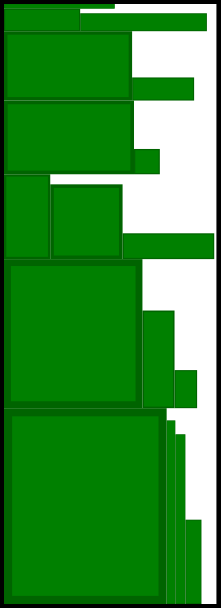
\includegraphics[width=.5\linewidth]{FFDHrun.png}
  \caption{FFDH Algorithm}
  \label{fig:ffdhrun}
\end{subfigure}%
\begin{subfigure}{.35\textwidth}
  \centering
  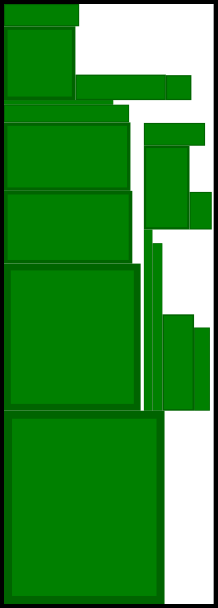
\includegraphics[width=.5\linewidth]{SplitFitrun.png}
  \caption{Split-Fit Algorithm}
  \label{fig:splitfitrun}
\end{subfigure}
  \caption{Visualisation for our implementation of FFDH and SF}
  \label{fig:ffdhsfrun}
\end{figure}

\noindent
Currently, we are in the process of implementing a Maximal Rectangles-based exhaustive (exponential) algorithm to solve 2-D Bin Packing, based on the idea that when the rectangles in any optimal packing are pushed towards the bottom-left corner of the strip, the packing becomes a solution that can be found by the maximal-rectangles exhaustive search that is no worse than the optimal solution (because we only push rectangles left and downwards).\\\
\\
With the use of FFDH and SF, we can then derive upper and lower bounds for the exhaustive search, from which we hope to create a branch-and-bound algorithm to solve 2-D Strip Packing.

\begin{thebibliography}{9}
\bibitem{harren1}
  Harren, R., Jansen, K., Pradel, L., van Stee, R.:
  \emph{A (5/3 + $\epsilon$)-Approximation for Strip Packing},
  In: WADS 2011 : Algorithms and Data Structures Symposium

\bibitem{baker1}
  Baker, B.S., Brown, D.J., Katseff, H.P.:
  \emph{A 5/4 algorithm for two-dimensional packing},
  Journal of Algorithms 2(4) (1981) 348–368
\end{thebibliography}

\end{document}